%!TEX root = ../thesis.tex
%*******************************************************************************
%****************************** Second Chapter *********************************
%*******************************************************************************

\chapter{Computational methods \label{chap:2}}

\ifpdf
    \graphicspath{{Chapter2/Figs/Raster/}{Chapter2/Figs/PDF/}{Chapter2/Figs/}}
\else
    \graphicspath{{Chapter2/Figs/Vector/}{Chapter2/Figs/}}
\fi

As mentioned in the last chapter, theories behind the calculations are the most crucial component in the material properties determination process. Its correctness, accuracy and implementation directly influence the quality of its prediction. In this chapter, I will introduction relevant theoretical models, approximation and their implementation in commonly used software packages.

\section{Theory}
\subsection{Density Functional Theory}

Density functional theory (DFT) is one of the most widely used method to calculation material properties. Its applicable length and time scale are in nanometer and picosecond. This is higher than quantum Monte Carlo simulation and lower than semi- or full-empirical methods in both scales. This order is also valid in the accuracy verse number-of-atoms-in-simulation plot in \autoref{fig:dft_ac}. It is reported that much of the inaccuracy attributes to the uncertainty of the experimental results that the methods are compared with\cite{Kirklin2015}. For periodic bulk or nanostructure, DFT can be used to even quantitatively predict the properties of materials. DFT
is based on two main basis: Hohenberg-Kohn theorems\cite{Hohenberg1964} and Kohn-Sham equations\cite{Kohn1965}. Here we briefly overview these without put too much effect for the derivation which have been extensively documented in other textbooks. 

\begin{figure}[htbp!] 
\centering  
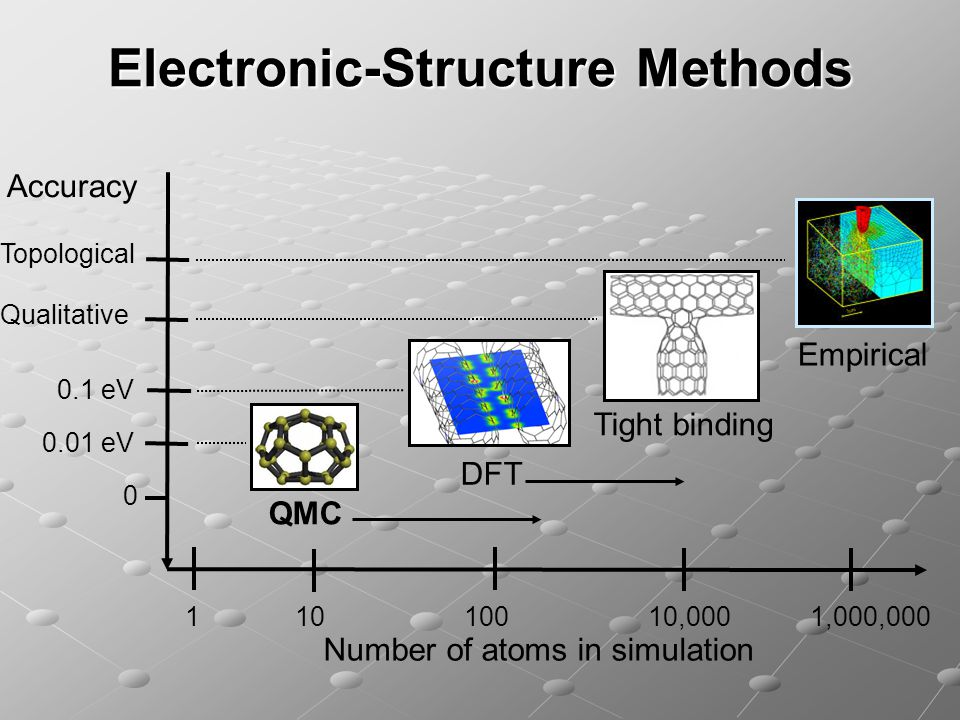
\includegraphics[width=0.7\textwidth]{dft1.jpg}
\caption{ Comparison of accuracy and capability of electronic structure calculation methods. Image source: \cite{dft_ac}.}  
\label{fig:dft_ac}
\end{figure} 

Materials are made from electrons and nuclei. Type of nuclei and interaction between these components give rise to various materials and their properties. The interactions are mainly electrostatic or Coulombic. While electrons must be described with quantum mechanics, the nuclei can be treated as classical particles. The equation governs electrons behaviours is the Schrödinger equation, it can be written as following\footnote{equations in this chapter are written in cgs form, and the fundamental constants $\hbar$, $e^2$ and $m$ are set to unity}

\begin{equation}
\begin{aligned}
\hat{H}\mathit{\Psi}_k(\vec{r_1}\sigma_1,\ldots,\vec{r_N}\sigma_N) &=\left[ -\frac{1}{2}\sum^N_{i=1}\nabla_i^2+\sum^N_{i=1}\upsilon(\vec{r}_i)+\frac{1}{2}\sum_{i=1}\sum_{j\neq i}\frac{1}{|\vec{r}_i-\vec{r}_j|}\right]\mathit{\Psi}_k(\vec{r_1}\sigma_1,\ldots,\vec{r_N}\sigma_N)  \\
&=\left( \hat{T} + \hat{V}_{ext} + \hat{V}_{ee}\right)\mathit{\Psi}_k(\vec{r_1}\sigma_1,\ldots,\vec{r_N}\sigma_N) \\
&=E_k\mathit{\Psi}_k(\vec{r_1}\sigma_1,\ldots,\vec{r_N}\sigma_N) .
\end{aligned}
\end{equation}

$\hat{H}$ is the total hamiltonian. $\hat{T}$ is the kinetic energy. $\hat{V}_{ext}$ is the interaction between electrons and nuclei. Here we already started with the first approximation: Born–Oppenheimer approximation\cite{Born1927}. Which neglect the dynamics of nuclei, instead electrons are moving in a static potential generated by their interaction with all nuclei. $\hat{V}_{ee}$ is interaction between electrons. The first two sum over all $N$-electrons, and the last sums over all unique pairs of $N$-electrons. $\vec{r}$ is the electron position. $\sigma$ is the z-component of spin on electron (+$\frac{1}{2}$,-$\frac{1}{2}$). $\mathit{\Psi}$ is the $N$-electron wave function, and it should be antisymmetric under interchange of two electron orbital and spin coordinates (fermionic character for electrons) and it should also satisfy boundary condition of the system (quantum confinement for low-dimensional system). $E$ is the total energy. $k$ is the complete set of $N$-electron quantum numbers. Following constrained search algorithm introduced by M. Levy\cite{Levy1979}, the ground-state energy $E$ can be found by minimizing the expected value of total hamiltonian with respect to wave function:

\begin{equation}
E=\min_\mathit{\Psi}\bra{\mathit{\Psi}}\hat{H}\ket{\mathit{\Psi}}.
\end{equation}

Here we take two steps for the minimization. For the first step, we minimize with respect to all wave functions gives the same density $n(\vec{r})$:

\begin{equation}
E=\min_{\mathit{\Psi}\rightarrow n}\bra{\mathit{\Psi}}\hat{T}+\hat{V}_{ee}\ket{\mathit{\Psi}}+\int dr^3\upsilon(\vec{r})n(\vec{r}).
\end{equation}

Then with the resulting wave function $\mathit{\Psi}^{min}_n$ that yields minimum $E$ and associate with density $n(\vec{r})$, we can construct universal functional:

\begin{equation}
\min_{\mathit{\Psi}\rightarrow n}\bra{\mathit{\Psi}}\hat{T}+\hat{V}_{ee}\ket{\mathit{\Psi}}=\bra{\mathit{\Psi}^{min}_n}\hat{T}+\hat{V}_{ee}\ket{\mathit{\Psi}^{min}_n}=F[n(\vec{r})]
\end{equation}

As seen in this equation, a functional, $F[n(\vec{r})]$, is a function of a function. For the second step, we minimized with respect to all densities $n(\vec{r})$:

\begin{equation}
E=\min_n \left\lbrace F[n(\vec{r})] + \int dr^3\upsilon(\vec{r})n(\vec{r}) \right\rbrace,
\end{equation}

where $\upsilon(\vec{r})$ is kept fix during minimization. The resulting density is the ground-state density that gives lowest ground state energy. This is known as density variational principle, also the main idea of the Hohenberg-Kohn theorems. For the completeness, they are present in the following:

\begin{theorem}

The external potential, $V_{ext}(\vec{r})$, of any system of interacting particles is uniquely determined (up to a constant) by the particle density, $n_0(\vec{r})$, of the ground state.

\end{theorem}

\begin{theorem}

The ground state energy of a system with an external potential $V_{ext}(\vec{r})$ is given by the minimum value of the energy functional $E_{HK} [n]$ and the density for which this minimum is reached corresponds with the ground state density $n_0(\vec{r})$.

\end{theorem}

Now, the main problem is to define the approximated expression of $F[n(\vec{r})]$. Kohn-Sham equation is a elegant way to do that. It aim to construct a non-interacting system, where density can be calculated exactly, and add local external potential $V_{KS}(\vec{r})$. The $F[n]$ decomposed into following and define $E_{EX}[n]$ as exchange-correlation (EX) energy:

\begin{equation}
F[n]=T_s[n]+E_H[n]+E_{EX}[n],
\end{equation}

where $T_s[n]$ is the non-interacting kinetic energy functional, and $E_H[n]$ is the Hartree energy functional:

\begin{equation}
E_H[n]=\frac{1}{2}\int d^3r\int d^3r\prime\frac{n(\vec{r})n(\vec{r\prime})}{|\vec{r}-\vec{r\prime}|}.
\end{equation}

Apart from the last term, $E_{EX}[n]$, everything else can be exactly calculated for non-interacting system for given density. By imposing a normalisation constraint on the electron density, $\int n(\vec{r})d\vec{r}=N$, we have

\begin{equation}
\frac{\delta F[n]}{\delta n(\vec{r})}=-\upsilon(\vec{r}).
\end{equation}

Therefore, the effective local potential, $V_{KS}(\vec{r})$, will be

\begin{equation}
V_{KS}(\vec{r})=\upsilon(\vec{r})+\frac{\delta E_H[n]}{\delta n(\vec{r})}+\frac{\delta E_{EX}[n]}{\delta n(\vec{r})},
\end{equation}

and the Kohn-Sham equation reads

\begin{equation}\label{eq:1}
\left[ -\frac{1}{2}\nabla_i^2+\upsilon(\vec{r})+\frac{\delta E_H[n]}{\delta n(\vec{r})}+\frac{\delta E_{EX}[n]}{\delta n(\vec{r})}\right]\mathit{\psi}_k(\vec{r}\sigma)=\varepsilon_k\mathit{\psi}_k(\vec{r}\sigma),
\end{equation}

and ground-state density is 

\begin{equation}\label{eq:2}
n(\vec{r})=\sum_k^{occ.}\sum_\sigma|\mathit{\psi}_k(\vec{r}\sigma)|^2.
\end{equation}

This can be solved self-consistently. An initial guess on the density $n(\vec{r})$ determines the effective potential $V_{KS}(\vec{r})$, from \eqref{eq:1} a wave function $\mathit{\psi}_k(\vec{r}\sigma)$ can be calculate, which will give a new density through \eqref{eq:2}. This procedure is repeated until self-consistency is reached. 

\subsection{Exchange-correlation functional}

The EX energy functional needs to be approximate. The choice of this directly influence the accuracy of the results. Since, although it is often the small fraction of the total energy, its contribution to chemical bonding and formation energy usually exclusive. The generalized gradient approximation (GGA) has become popular in solid state calculations. It is a further upgrade of its previous version, the local density approximation (LDA). The LDA has the following form:

\begin{equation}
E_{XC}^{LDA}[n]=\int n(\vec{r})\epsilon_{XC}[n(\vec{r})]d\vec{r}.
\end{equation}

$\epsilon_{XC}[n(\vec{r})]$ is the EX energy for homogeneous electron gas having density of $n(\vec{r})$, and it is usually taken from Quantum Monte Carlo calculations. Whereas the GGA further includes the derivative of density, $\nabla n(\vec{r})$, as an argument for $\epsilon_{XC}$, thus it reads

\begin{equation}
E_{XC}^{GGA}[n]=\int \epsilon_{XC}[n(\vec{r}),\nabla n(\vec{r})]d\vec{r}.
\end{equation}

Contrast to LDA, there is no unique input for $\epsilon_{XC}(n(\vec{r}),\nabla n(\vec{r})$. 

\section{Implementation}
\subsection{Basis set, Plane wave energy cut-off, K-points}
\subsection{Software Packages}